\newpage
\section{Durchführung}
    \subsection{Versuchsaufbau}
        \begin{figure}[h]
          \centering
          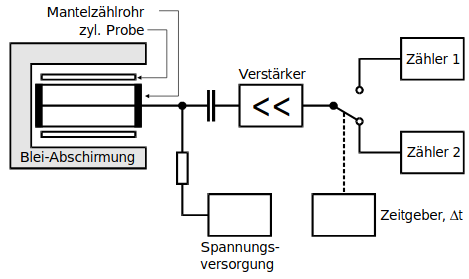
\includegraphics[width = 0.6\textwidth]{pictures/Aufbau.png}
          \caption{Hier ist der Aufbau der Versuchsschaltung dargestellt. Entnommen aus \cite{tu_dortmund_versuchsanleitung_2021-1}}
          \label{fig:Aufbau}
        \end{figure}

        \FloatBarrier

        An den Szintillator sind zwei Photomultiplier (PMT) angeschlossen, um mögliche Störungen, die an nur einem PMT in die Messung einfließen können mithilfe der Koinzidenz auszuschließen.
        Damit die Signale möglichst zeitgleich an der Koinzidenz ankommen werden hinter die PMTs Verzörgerungsleitungen, die aus Kabelspulen bestehen, dazugeschaltet.
        Die Diskriminatoren filtern je nach eingestellter Schwelle Signale.
        Wie schon erwähnt lässt die Koinzidenz nur ein Signal durch, wenn alle Input-Signale in einer bestimmten Auflösungszeit ankommen.

        Anschließend ist eine, durch eine elektronische Schaltung realisierte, Stoppuhr aufgebaut. Die Koinzidenz ist über eine weitere Verzörgerungsleitung und eine monostabile Kippstufe (Monoflop) an zwei AND-Gatter angeschlossen. Diese sind mit einem Time-Amplitude-Converter (TAC) verbunden, welcher selbst an einen Vielkanalanalysator (Multi-Channel-Analyser, MCA) angeschlossen ist. Ein Computer liest diesen aus und speichert die gemessenen Daten.

        Außerdem wird ein Doppelimpulsgenerator zur Kalibrierung des MCA und zwei Impulszähler zum zählen der Start- und Stoppsignale benötigt.

    \subsubsection*{Wirkungsweise der Stoppuhr-Schaltung}
        Zuerst wird die Funktionsweise eines Monoflop beschrieben: \\
        Solange er nicht getriggert wird, gibt der Monoflop ein Signal aus seinem negativen Output aus.
        Wird er getriggert wird das gesendete Signal über einen eingestellten Zeittraum, die Suchzeit $T_{\text{S}}$, vom negativen zum positiven Output gewechselt. Während dieser Suchzeit bewirken ankommende Signale keine Änderungen am Monoflop.

        Die Koinzidenz gibt ein erstes Signal aus. Dieses erreicht einerseits das 1. AND-Gatter als auch mit einer Verzörgerung von $30$ns den Monoflop, der dem 1. AND-Gatter ein negatives Signal sendet. Das führt zu einem Startsignal am TAC. Nach der Verzörgerung von $30$ns wechselt der Monoflop vom negativen auf den positiven Output, blockiert damit das 1. AND-Gatter, sodass es während der Suchzeit kein weiteres Startsignal abschicken kann und ermöglicht dem 2. AND-Gatter ein Stoppsignal zu senden. \\
        Gibt die Koinzidenz jetzt während der Suchzeit ein zweites Signal aus, erreicht dieses das 2. AND-Gatter und das Stoppsignal wird gesendet. Kommt das zweite Signal nicht während der Suchzeit an wird es als erstes Signal behandelt, da sich der Monoflop wieder zurückgesetzt hat. Die Verzörgerungszeit wird viel kleiner als die durchschnittliche Zeit die ein weiteres Myon braucht um anzukommen gewählt, da es dann sehr unwahrscheinlich ist, dass in dieser Zeit ein Myon ankommt und ein zusätzliches Startsignal senden kann.

    \subsection{Versuchsdurchführung}
        Als ersten Schritt wird durch Anschließen eines Oszillokops die Funktionstüchtigkeit der PMTs überprüft. Danach werden die Diskriminatoren angeschlossen und jeweils mithilfe eines Impulszählers so geregelt, dass ca. 30 Impulse pro Sekunde gemessen werden. Praktisch wird z.B. 10 Sekunden gemessen, sodass ca. 300 Impulse am Impulszähler abgelesen werden.

        Zur Justage der Verzörgerungsleitungen werden die Impulse hinter der Koinzidenz abgelesen, während die Differenz zwischen den Verzörgerungsleitungen systematisch in 1ns-Schritten verändert wird. Anschließend wird der weitere Versuch mit der Verzörgerung mit der höchsten Ereignisrate weitergeführt.

        Die restliche Schaltung wird aufgebaut, wobei am Monoflop eine Suchzeit von $T_{\text{S}} = 10 \, \mu$s eingestellt wird. \\
        Als Nächstes wird die Kalibration des MCA vorgenommen. Dazu wird der Aufbau bis einschließlich der Koinzidenz durch einen Doppelimpulsgenerator ersetzt und es werden mindestens 10 Messwerte mit einem Impulsabstand im Bereich von $0,3 \, \mu$s bis $9,9 \, \mu$s aufgenommen.

        Nach Abschluss der Kalibration wird der Doppelimpulsgenerator wieder mit dem eigentlichen Aufbau getauscht und die Messung wird über einen Zeitraum von mehreren Tagen durchgeführt. \cite{tu_dortmund_versuchsanleitung_2021-1}
